\newpage
\criteria{Teaching and Learning Approach}

\subcriteria{The educational philosophy is shown to be articulated and communicated to all stakeholders. It is also shown to be reflected in the teaching and learning activities.}

ปรัชญาการศึกษาของมหาวิทยาลัยเทคโนโลยีราชมงคลธัญบุรี 
\begin{center}
	``นวัตกรรมสร้างชาติ ราชมงคลธัญบุรีสร้างนวัตกรรม''
\end{center}
\indent\indent ปรัชญาดังกล่าวถูกสื่อสารไปยังกลุ่มผู้มีส่วนได้ส่วนเสียที่สำคัญ และมีการประเมินการรับรู้ดังตาราง \ref{Table:SH}

\begin{longtable}{|>{\raggedright}p{0.3\textwidth}|>{\raggedright\arraybackslash}p{0.38\textwidth}|>{\raggedright\arraybackslash}p{0.3\textwidth}|}
    \caption{ช่องทางการสื่อสารและผลการรับรู้ ``ปรัชญาการศึกษา" ของกลุ่มผู้มีส่วนได้ส่วนเสีียที่สำคัญ}
    
    \label{Table:SH}    \\
    \hline
    \multicolumn{1}{|c|}{\bf ผู้มีส่วนได้ส่วนเสีย}&\multicolumn{1}{c|}{\bf ช่องทางการสื่อสาร}&\multicolumn{1}{c|}{\bf ร้อยละของการรับรู้ปรัชญาการศึกษา}\\
    \hline
    \endhead
    %\multicolumn{2}{|l|}{\textbf{ผู้มีส่วนได้ส่วนเสียภายนอก (External Stakeholders)}} \\ \hline
    ผู้ใช้บัณฑิต/สถานประกอบการ & หนังสือประชาสัมพันธ์หลักสูตร & \multicolumn{1}{c|}{100} \\ \hline
    ผู้สนใจสมัครเข้าศึกษาในหลักสูตร & 
    เว็บไซต์ของมหาวิทยาลัย คณะ และสาขาวิชา
    & \multicolumn{1}{c|}{81.81 } \\ \hline
    %\multicolumn{2}{|l|}{\textbf{ผู้มีส่วนได้ส่วนเสียภายใน (Internal Stakeholders)}} \\ \hline
    %มหาวิทยาลัย/คณะฯ & \printprogram{} (มคอ. 2) &  \multicolumn{1}{c|}{100}  \\ \hline
    อาจารย์ผู้รับผิดชอบหลักสูตร และอาจารย์ผู้สอน & การประชุมอาจารย์ผู้รับผิดชอบหลักสูตร และอาจารย์ผู้สอน &  \multicolumn{1}{c|}{100}  \\ \hline
    นักศึกษา & 
    \begin{enumerate}[label=-] \vspace{-0.7cm}
    	\item เว็บไซต์ของมหาวิทยาลัย คณะ และสาขาวิชา
    	\item อาจารย์ที่ปรึกษา 
    	\item คู่มือนักศึกษา    
    \end{enumerate}
    &  \multicolumn{1}{c|}{100}  \\ \hline
    ผู้ปกครอง & 
    ประชุมผู้ปกครอง
    &  \multicolumn{1}{c|}{100}  \\ \hline
\end{longtable}

	


%\noindent\textbf{การสื่อสารและทำความเข้าใจปรัชญาการศึกษา}\\
%
%ปรัชญา ``นวัตกรรมสร้างชาติ ราชมงคลธัญบุรีสร้างนวัตกรรม" ได้รับการเผยแพร่ผ่านช่องทางต่างๆ ของมหาวิทยาลัย เช่น เว็บไซต์ สื่อประชาสัมพันธ์ การประชุม และการปฐมนิเทศนักศึกษาใหม่ คณาจารย์และบุคลากรทุกคนได้รับการปลูกฝังให้เข้าใจถึงความสำคัญของนวัตกรรมในการพัฒนาประเทศ และบทบาทของมหาวิทยาลัยในการสร้างสรรค์นวัตกร โดยเฉพาะในหลักสูตรได้สื่อสารปรัชญาการศึกษากับอาจารย์ผู้สอนให้รับทราบแนวทางการจัดการเรียนการสอนที่มุ่งเน้นการพัฒนาบัณฑิต
%สู่การเป็นนวัตกร ผ่านการประชุมอาจารย์ผู้รับผิดชอบหลักสูตร และอาจารย์ผู้สอน มีการเน้นย้ำว่าคณิตศาสตร์ประยุกต์เป็นเครื่องมือสำคัญในการสร้างสรรค์นวัตกรรมในหลากหลายสาขา การสะท้อนปรัชญาในกิจกรรมการเรียนการสอน

นอกจากนี้หลักสูตรได้นำปรัชญาการศึกษาของมหาวิทยาลัยเทคโนโลยีราชมงคลธัญบุรี ไปใช้ในการจัดการเรียนการสอน  ดังนี้
\begin{enumerate}
	\item การส่งเสริมการจัดการเรียนรู้แบบ Active Learning  \\อาจารย์ในหลักสูตรส่งเสริมการเรียนรู้ที่เน้นให้นักศึกษาเป็นศูนย์กลาง มีการจัดกิจกรรมที่กระตุ้นให้นักศึกษาคิดวิเคราะห์ แก้ปัญหา และสร้างสรรค์สิ่งใหม่ๆ เช่น การทำโครงงานกลุ่ม การนำเสนอผลงาน การอภิปรายแลกเปลี่ยนความคิดเห็น การจัดทำกรณีศึกษา (Case Study) ที่เกี่ยวข้องกับการประยุกต์ใช้คณิตศาสตร์เพื่อแก้ไขปัญหาทางอุตสาหกรรมธุรกิจ วิทยาศาสตร์ หรือวิศวกรรมศาสตร์
	\item การบูรณาการเทคโนโลยีและนวัตกรรมในการเรียนการสอน \\มีการนำเครื่องมือและซอฟต์แวร์ทางคณิตศาสตร์ที่ทันสมัยมาใช้ในการเรียนการสอน เช่น Python เพื่อให้นักศึกษาสามารถนำความรู้ทางคณิตศาสตร์ไปประยุกต์ใช้ในการสร้างสรรค์นวัตกรรม และพัฒนาทักษะที่จำเป็นในยุคดิจิทัล นอกจากนี้ยังมีการส่งเสริมให้นักศึกษาเข้าร่วมการแข่งขันทางคณิตศาสตร์ประยุกต์
	\item การส่งเสริมคุณลักษณะของนวัตกร \\นอกเหนือจากความรู้และทักษะทางวิชาการ หลักสูตรยังเน้นการปลูกฝังคุณลักษณะที่จำเป็นสำหรับนวัตกร เช่น ความคิดสร้างสรรค์ การแก้ปัญหา ความสามารถในการทำงานร่วมกับผู้อื่น การปรับตัว ซึ่งสะท้อนผ่านกิจกรรมการเรียนการสอนที่เปิดโอกาสให้นักศึกษาได้ลงมือปฏิบัติจริง  
\end{enumerate}


%\newpage
\begin{doclist}
	\docitem{รายงานผลการรับรู้ปรัชญาการศึกษาของ มทร.ธัญบุรี}
	%\docitem{การสื่อสารปรัชญาการศึกษากับนักศึกษา}
	%\docitem{ช่องทางการสื่อสารกับผู้มีส่วนได้ส่วนเสีย}
\end{doclist}

%\newpage
\subcriteria{The teaching and learning activities are shown to allow students to participate responsibly in the learning process.}

%%%%%%%%%%%%
การจัดการเรียนการสอนในหลักสูตรเปิดโอกาสให้นักศึกษามีส่วนร่วมรับผิดชอบในกระบวนการเรียนรู้ เช่น

\begin{enumerate}
    \item รายวิชาสัมมนาทางคณิตศาสตร์ประยุกต์ และรายวิชาโครงงานด้านคณิตศาสตร์ประยุกต์  \\ให้นักศึกษามีส่วนร่วมรับผิดชอบในกระบวนการเรียนรู้  ดังนี้    
   \begin{itemize}
        \item เลือกหัวข้อสัมนาและหัวข้อโครงงานที่สนใจที่จะศึกษาและเสนอต่ออาจารย์ที่ปรึกษาโครงงาน
        \item เลือกอาจารย์ที่ปรึกษาสัมนาและอาจารย์ที่ปรึกษาโครงงาน
        \item กำหนดวางแผนตารางเวลาและกำหนดกิจกรรมร่วมกัน
    \end{itemize}
    \item รายวิชาการตัดสินใจอย่างชาญฉลาดด้วยกำหนดการเชิงคณิตศาสตร์ \\ให้นักศึกษามีส่วนร่วมรับผิดชอบในกระบวนการเรียนรู้  โดยเปิดโอกาสให้นักศึกษาเลือกปัญหาที่เป็นไปได้จากสถานการณ์จริง และออกแบบวิธีการแก้ปัญหาด้วยตนเองพร้อมนำเสนอ
    \item รายวิชาทักษะการนำเสนอผลงานทางด้านคณิตศาสตร์ \\ให้นักศึกษามีส่วนร่วมรับผิดชอบในกระบวนการเรียนรู้  ดังนี้  
%    ให้นักศึกษา เลือกหัวข้อ ประเมินเพื่อน
    \begin{itemize}
    	\item มีส่วนร่วมในการวางแผนกิจกรรมการเรียนการสอนและประเมินผล
    	\item เลือกหัวข้อทางด้านคณิตศาสตร์ที่สนใจ และนำเสนอ
    	\item มีส่วนร่วมในการประเมินผลการนำเสนอของเพื่อนร่วมชั้นเรียน
    \end{itemize}
   

   \end{enumerate}
%%%%%%%%%%%%%%%%%%%%%%%%%
\begin{doclist}
	\docitem{รายละเอียดของรายวิชา (มคอ.3) รายวิชาสัมมนาทางคณิตศาสตร์ประยุกต์}
	\docitem{รายละเอียดของรายวิชา (มคอ.3) รายวิชาโครงงานด้านคณิตศาสตร์ประยุกต์}	
	\docitem{รายละเอียดของรายวิชา (มคอ.3) รายวิชาการตัดสินใจอย่างชาญฉลาดด้วยกำหนดการเชิงคณิตศาสตร์}
	\docitem{รายละเอียดของรายวิชา (มคอ.3) รายวิชาทักษะการนำเสนอผลงานทางด้านคณิตศาสตร์}
	%\docitem{การมีส่วนร่วมในกระบวนการเรียนรู้ของนักศึกษา}
\end{doclist}
\newpage
%%%%%%%%%%%%%%%%%%%%
\subcriteria{The teaching and learning activities are shown to involve active learning by the students.}
ทุกรายวิชาที่เปิดสอนในปีการศึกษา 2567 มีการออกแบบและจัดกิจกรรมการเรียนการสอนที่ส่งเสริมการเรียนรู้เชิงรุก (Active Learning) ซึ่งมีรายละเอียดดังตาราง \ref{table3.3}
%%%%%%%%%%%%%%%%%%%%%%%%%%%%%%%%%%%%%%%%%%%%%%%
{\small
	\begin{center}
		\begin{longtable}{|p{0.08\textwidth}|p{0.1\textwidth}|p{0.15\textwidth}|>{\raggedcolumns}p{0.58\textwidth}|}
			\caption{รูปแบบของการจัดการเรีนการสอนแบบ Active Learning ของรายวิชาในปีการศึกษา 2567}
			\label{table3.3}
			\\
			\hline
			\multicolumn{1}{|c|}{\textbf{ภาคเรียน}} &
			\multicolumn{1}{c|}{\textbf{รหัสวิชา}} &
			\multicolumn{1}{c|}{\textbf{ชื่อวิชา}} &
			\textbf{รูปแบบของการจัดการเรีนการสอนแบบ Active Learning}\\
			\hline
			\endfirsthead	
				\caption{(ต่อ) รูปแบบของการจัดการเรีนการสอนแบบ Active Learning ของรายวิชาในปีการศึกษา 2567 }\\
				\hline
			\multicolumn{1}{|c|}{\textbf{ภาคเรียน}} &
			\multicolumn{1}{c|}{\textbf{รหัสวิชา}} &
			\multicolumn{1}{c|}{\textbf{ชื่อวิชา}} &
			\textbf{รูปแบบของการจัดการเรีนการสอนแบบ Active Learning}\\
			\hline
			\endhead	
				\hline
				\endfoot
		1/2567&
	09111151&
	แคลคูลัส 1&
	\underline{การเรียนรู้ Active Learning แบบ Problem-Based Learning} โดยนักศึกษาสามารถจำสูตร เข้าใจและสามารถคิดวิเคราะห์โจทย์และการประยุกต์ใช้ความรู้กับโจทย์ปัญหาเกี่ยวกับอัตราสัมพัทธ์ โดยแบ่งกลุ่มนักศึกษาแต่ละกลุ่มวิเคราะห์โจทย์ เขียนแผนผังและสูตรที่เกี่ยวข้อง หาความสัมพันธ์ แสดงวิธีการแก้ปัญหาพร้อมนำเสนอ  	 
	\\ \cline{2-4}
	
	&09111253 &
	แคลคูลัส 3 &
	\underline{การเรียนรู้  Active Learning แบบ Thinking-Based Learning} เน้นให้ผู้เรียนฝึกกระบวนการคิดวิเคราะห์ผ่านบริบทของบทเรียนที่มีความซับซ้อนมากขึ้น เพื่อฝึกทักษะการคิดวิเคราะห์ (Critical Thinking), การคิดเป็นระบบ (Systematic Thinking), การคิดสร้างสรรค์ (Creative Thinking) โดยผู้เรียนเป็นศูนย์กลางของกระบวนการเรียนรู้ โดยลงมือคิด ตัดสินใจ และอธิบายกระบวนการ \\ \cline{2-4}
	
	&09113201&
	หลักคณิตศาสตร์&
	 \underline{การเรียนรู้ Active Learning แบบ Problem-Based Learning } \underline{Collaborative Learning และ Inquiry-Based Learning} มีกิจกรรมการเรียนการสอนที่ส่งเสริมให้นักศึกษาได้ฝึกทักษะกระบวนการคิดเชิงตรรกะ การให้เหตุผล และแก้ปัญหา โดยให้นักศึกษาฝึกการให้เหตุผล ฝึกแก้โจทย์ปัญหาด้วยตนเองทั้งเดี่ยว/กลุ่ม และให้นำเสนอหน้าชั้นเรียนให้เพื่อนร่วมชั้นเรียนร่วมแสดงความคิดเห็นและซักถาม โดยผู้สอนมีบทบาทเป็นผู้ให้คำแนะนำให้คำปรึกษา \\ \cline{2-4}
		
	& 09113305
	& การวิเคราะห์เชิงคณิตศาสตร์ & \underline{การเรียนรู้ Active Learning แบบ Problem-Based Learning } \underline{Collaborative Learning และ Inquiry-Based Learning} มีกิจกรรมการเรียนการสอนที่ส่งเสริมให้นักศึกษาได้ฝึกทักษะกระบวนการคิด การวิเคราะห์และแก้ปัญหา โดยให้นักศึกษาฝึกแก้โจทย์ปัญหาด้วยตนเองทั้งเดี่ยว/กลุ่ม และให้นำเสนอหน้าชั้นเรียนให้เพื่อนร่วมชั้นเรียนร่วมแสดงความคิดเห็นและซักถาม โดยผู้สอนมีบทบาทเป็นผู้ให้คำแนะนำให้คำปรึกษา 
	\\ \cline{2-4}
	
	& 09114205
	& กำหนดการเชิงคณิตศาสตร์เบื้องต้น &1. \underline{การเรียนรู้ Active Learning แบบ Brainstorming}\newline กิจกรรมให้นักศึกษาวิเคราะห์สถานการณ์จำลองด้วยกำหนดการเชิงคณิตศาสตร์และกำหนดตัวแปรในการสร้างแบบจำลองคณิตศาสตร์ (Brainstorming) \newline
	2. \underline{การเรียนรู้ Active Learning แบบ Cased-Based Learning} และ Problem-Based Learning กิจกรรมให้นักศึกษาแบ่งกลุ่มเพื่อกำหนดสถานการณ์จำลองกำหนดการเชิงคณิตศาสตร์และกำหนดตัวแปรด้วยตนเอง พร้อมหาผลเฉลยคำตอบและนำเสนอผลงาน 
	
	\\ 	
\cline{2-4}
	& 09114222
	& ระเบียบวิธีเชิงตัวเลขเบื้องต้น & 1. \underline{การเรียนรู้ Active Learning แบบ Project-Based}\newline \underline{Learning}
	\begin{itemize}
		\item ให้นักศึกษาแก้ปัญหาโจทย์จากสถานการณ์จริง เช่น สมการไม่เชิงเส้น ระบบสมการเชิงเส้น หรือการประมาณค่า
		\item ใช้ข้อมูลจากแหล่งจริง เช่น อุณหภูมิ ราคาเหรียญคริปโต หรือข้อมูลชีวภาพ มาฝึกวิเคราะห์
		\item 	ส่งเสริมให้เกิดการคิดเชิงระบบและเชิงตรรกะเพื่อหาวิธีแก้ที่มีประสิทธิภาพ
	\end{itemize}	
	\\
&&&	
	2.  \underline{การเรียนรู้ Active Learning แบบ Project-Based}\newline \underline{Learning}
	\begin{itemize}
		\item มอบหมายงานโค้ดโปรแกรมเพื่อแก้ปัญหาทางตัวเลข เช่น การเปรียบเทียบวิธี Newton-Raphson กับ Secant
		\item มีการสรุปผล วิเคราะห์จุดแข็ง/จุดอ่อนของแต่ละวิธี และอภิปรายร่วมกับกลุ่ม
		\item ผลลัพธ์นำเสนอผ่านรายงานหรือการนำเสนอในชั้นเรียน	
	\end{itemize}	
	\\
	&&&	
	3.  \underline{การเรียนรู้ Active Learning แบบ Project-Based}\newline \underline{Learning}
	\begin{itemize}
		\item นำงานวิจัยเกี่ยวกับ error analysis หรือ algorithm efficiency มาใช้เป็นกรณีศึกษา
		\item ฝึกใช้แนวทางวิจัยและการตั้งคำถามทางวิทยาศาสตร์
	\end{itemize}	
		\\
	&&&	
	4.  \underline{การเรียนรู้ Active Learning แบบ Collaborative }\newline \underline{Learning}
	\begin{itemize}
		\item จัดให้นักศึกษาแบ่งกลุ่มทำงาน เขียนโค้ดร่วมกัน และช่วยกันอภิปรายวิเคราะห์ผล
		\item ส่งเสริมทักษะการทำงานเป็นทีม การรับฟัง และการให้ feedback
		\item มีการอภิปรายแบบกลุ่มและการนำเสนอหน้าชั้น
	\end{itemize}	

	5.  \underline{การเรียนรู้ Active Learning แบบ Coaching/Mentoring }
	\begin{itemize}
		\item อาจารย์ทำหน้าที่โค้ช ให้คำแนะนำแบบตัวต่อตัวหรือกลุ่มเล็กระหว่างการทำกิจกรรม
		\item ช่วยแก้ปัญหาเชิงเทคนิค เช่น syntax error หรือการตั้งสูตรที่ผิด
		\item กระตุ้นให้นักศึกษาคิดด้วยตนเองก่อนให้คำตอบ
	\end{itemize}	
	\\ 	
	& 	& & 
	6.  \underline{การเรียนรู้ Active Learning แบบ Reflective Learning }
	\begin{itemize}
		\item วิเคราะห์ว่าเรียนรู้อะไรจากกิจกรรม coding หรือกรณีศึกษานั้นเสริมสร้างทักษะการคิดย้อนทวน (metacognition)
		\item ช่วยแก้ปัญหาเชิงเทคนิค เช่น syntax error หรือการตั้งสูตรที่ผิด
	\end{itemize}							
	%%%%%%%%%%%%
%	\\ 
%	\cline{2-4}
	\\ \cline{2-4}
	& 09114318
	& คณิตศาสตร์การเงิน & \underline{การเรียนรู้ Active Learning แบบ Project-Based}\newline \underline{Learning}
	โดยในหัวข้อการคำนวณอัตราดอกเบี้ย ซึ่งมีกรณีที่ซับซ้อนและคำนวณยาก ต้องใช้โปรแกรมมาช่วยในการคำนวณ มีการกำหนดปัญหาและให้นักศึกษาแบ่งเป็นกลุ่มเพื่อแก้ปัญหา โดยมีการใช้โปรแกรมทางคณิตศาสตร์มาแก้ปัญหา พร้อมทั้งมีการนำเสนอและอภิปรายหน้าชั้นเรียน
	\\ 
	\cline{2-4}
	& 09114335
	& ระบบฐานข้อมูล & 1. \underline{การเรียนรู้ Active Learning แบบ Project-Based}\newline \underline{Learning} \newline
	2. \underline{การเรียนรู้ Active Learning แบบ Case Studies} ใช้กรณีศึกษาในการอภิปรายในชั้นเรียน โดยเน้นให้นักศึกษาเรียนรู้จากสถานการณ์จริงหรือจำลองที่เกี่ยวข้องกับการใช้ระบบฐานข้อมูล เพื่อฝึกการวิเคราะห์ ออกแบบ และเสนอแนวทางแก้ปัญหาจริง
	\\ 
	\cline{2-4}
	& 09114338
	& การพัฒนาเว็บไซต์สมัยใหม่ &1. \underline{การเรียนรู้ Active Learning แบบ Project-Based}\newline \underline{Learning}
	\begin{itemize}
		\item นักศึกษาได้รับโจทย์ให้พัฒนาเว็บแอปพลิเคชันแบบครบวงจร (Full-stack project) เช่น ระบบจัดการผู้ใช้ ระบบแสดงข้อมูล หรือเว็บบล็อก
		\item ใช้เทคโนโลยีทั้งด้าน frontend (React.js) และ backend (Node.js + MongoDB)
		\item การประเมินผ่านการพัฒนาโครงงานจริง โดยใช้เวิร์กช็อปทุกสัปดาห์เป็นส่วนหนึ่งของการพัฒนาอย่างต่อเนื่อง
	\end{itemize} 
	\\ 	
	& 	& & 
		2. \underline{การเรียนรู้ Active Learning แบบ Project-Based}\newline \underline{Learning}\newline สัปดาห์ที่เกี่ยวกับการทำ RESTful AP Authentication และ Performance Optimization มีโจทย์จริงให้แก้ เช่น สร้างระบบล็อกอินและการควบคุมสิทธิ์เข้าถึง การปรับปรุงความเร็วในการโหลดเว็บไซต์ นักศึกษาต้องวิเคราะห์ปัญหา ออกแบบวิธีการ และทดสอบแนวทางของตนเอง \\	& 	& & 
	3. \underline{การเรียนรู้ Active Learning แบบ Collaborative}\newline \underline{Learning}
	\begin{itemize}
		\item มีการแบ่งกลุ่มให้นักศึกษาร่วมกันพัฒนาโปรเจกต์ เช่น ตั้ง GitHub repository ร่วมกันในสัปดาห์ Git and GitHub
		\item ใช้ Git flow เป็นรูปแบบการจัดการทีมจริงในการเขียนโค้ด
		\item การอภิปรายเชิงเทคนิคในการนำเสนองานและรับฟังคำติชม
	\end{itemize}
   \\	& 	& & 
    4. \underline{การเรียนรู้ Active Learning แบบ Case-Based}\newline \underline{Learning}
    \begin{itemize}
    	\item ยกตัวอย่างเว็บไซต์จริง (เช่น Netflix Lazada หรือ Google Maps) มาให้ศึกษาวิเคราะห์โครงสร้างและเทคนิคการเขียน
    	\item ให้เปรียบเทียบและจำลองฟังก์ชันบางอย่าง เช่น ระบบการกรอกฟอร์ม ระบบค้นหา หรือการเรียก API ด้วย AJAX
    \end{itemize}
   \\	& 	& & 
     5. \underline{การเรียนรู้ Active Learning แบบ Reflective }\newline \underline{Learning}
    \begin{itemize}
    	\item นักศึกษาต้องจัดทำเอกสารสรุป (Project Documentation หรือ README.md) เพื่ออธิบายโครงสร้าง ระบบงาน และสิ่งที่ได้เรียนรู้
    	\item มีการนำเสนอผลงาน พร้อมทั้ง feedback ว่าแต่ละคนมีการเติบโตทางความคิดหรือทักษะอย่างไร
    \end{itemize}

    \\ 	
    & 	& & 
     6. \underline{การเรียนรู้ Active Learning แบบ Coaching/Mentoring }
    \begin{itemize}
    	\item ผู้สอนให้คำแนะนำรายบุคคลและแบบกลุ่มเล็กในช่วง Workshop
    	\item ช่วย debug แก้ปัญหาการเชื่อมต่อ API deploy หรือจัดการฐานข้อมูล MongoDB และ Mongoose
    	\item ส่งเสริมให้นักศึกษาเป็นผู้เรียนรู้เชิงรุก (self-directed learner)
    \end{itemize}
 	\\
	\cline{2-4}
	& 09116402
	& สหกิจศึกษาทางคณิตศาสตร์ & 1. \underline{การเรียนรู้ Active Learning แบบ Experiential}\newline \underline{Learning} นักศึกษาได้ลงมือปฏิบัติงานจริงในสถานประกอบการ เสมือนเป็นพนักงานเต็มตัว ในตำแหน่งตามที่ตรงกับสาขาวิชาและเหมาะสมกับความรู้ความสามารถ เป็นระยะเวลาไม่น้อยกว่า 16 สัปดาห์ ปฎิบัติตนตามระเบียบซึ่งถือเป็นหัวใจของ Experiential Learning โดยเน้นการเรียนรู้ผ่านการกระทำ และการสะท้อนคิด  (Reflection)\newline 
	2. \underline{การเรียนรู้ Active Learning แบบ Project-Based}\newline \underline{Learning} สำหรับนักศึกษาบางกลุ่มสามารถสร้างผลงานในรูปแบบโครงงานได้ บางกลุ่มมีโอกาสนำปัญหาจริงในสถานประกอบการ มาวิเคราะห์ ออกแบบ และพัฒนาเป็นโครงงาน ซึ่งสอดคล้องกับการเรียนรู้แบบใช้โครงงานเป็นฐาน
	\\ \cline{2-4} 
	 & 09116406
	& ปัญหาพิเศษจากสถานประกอบการ ทางคณิตศาสตร์ประยุกต์ & \underline{การเรียนรู้ Active Learning แบบ Experiential}\newline \underline{Learning และ Inquiry-Based Learning} โดยให้นักศึกษานำหัวข้อที่สนใจจากที่ได้ฝึกงานในสถานประกอบการมาทำโปรเจค โดยอาจารย์มีบทบาทเป็นผู้ให้คำแนะนำปรึกษา
	\\ \hline
	 2/2567& 09111152 & แคลคูลัส 2& \underline{การเรียนรู้ Active Learning แบบ Thinking Based}\newline
	\underline{Learning Case Study} ผู้สอนจัดการเรียนการสอนโดยนำระบบคอมพิวเตอร์พีคณิตมาใช้ นำตำราภาษาอังกฤษมาใช้ในบางหัวข้อและนำงานวิจัยของอาจารย์มาเป็นกรณีศึกษา
		\\
	\cline{2-4}
	& 09111257 & สมการเชิงอนุพันธ์สามัญ& \underline{การเรียนรู้ Active Learning แบบ Blended Active}\newline \underline{Learning Problem-Based Learning}\newline และ \underline{Collaborative Learning}  โดยมุ่งส่งเสริมการมีส่วนร่วมของนักศึกษาในการเรียนรู้ผ่านกระบวนการปฏิบัติจริง การอภิปราย และการแลกเปลี่ยนแนวคิดทางคณิตศาสตร์อย่างมีระบบ
	\newline - ดำเนินการสอนผ่านการ บรรยายเชิงทฤษฎี เพื่อปูพื้นฐานความรู้เกี่ยวกับสมการเชิงอนุพันธ์สามัญ ทั้งในด้านแนวคิดสำคัญ คุณสมบัติของสมการ วิธีการหาคำตอบ และการวิเคราะห์พฤติกรรมของคำตอบ 
	\newline - กิจกรรมปฏิบัติการ เพื่อให้นักศึกษาฝึกใช้ทฤษฎีในการแก้ไขปัญหาทางคณิตศาสตร์ที่ใกล้เคียงกับสถานการณ์จริง ตลอดจนสามารถประยุกต์ใช้เครื่องมือเชิงวิเคราะห์ในการตีความผลลัพธ์ที่ได้ 
	\\ 
	\cline{2-4}
	& 09113114 & วิยุตคณิต&
	\underline{การเรียนรู้ Active Learning แบบ Collaborative  Learning}\newline \underline{Problem-Based Learning Discovery Learning และ} \underline {Presentation-Based Learning}  โดยแบ่งกลุ่มนักศึกษา ศึกษาปัญหาหอคอยฮานอย สร้างความสัมพันธ์เวียนเกิด พร้อมทั้งนำเสนอ \\
	\cline{2-4}
	& 09113202 & พีชคณิตเชิงเส้น&
	\underline{การเรียนรู้ Active Learning แบบ Collaborative  Learning}\newline \underline{Problem-Based Learning Discovery Learning และ} \underline {Presentation-Based Learning} โดยแบ่งกลุ่มนักศึกษา ศึกษาโจทย์ปัญหาเกี่ยวกับระบบสมการเชิงเส้น 2 ตัวแปร 2 สมการ วิธีการแก้ปัญหา พร้อมทั้งนำเสนอ  
	\\ 
	\cline{2-4}
	& 09113306 & พีชคณิตนามธรรม&
	การเรียนรู้ \underline{Active Learning แบบ Thinking Based Learning} \underline{case Study และ Academic Reading-Based Learning} โดยได้นำงานวิจัยของอาจารย์มาเป็นกรณีศึกษาในหัวข้อเรื่องกรุปและนำตำราภาษาอังกฤษมาใช้ในบางหัวข้อเพื่อให้นักศึกษาเตรียมพร้อมสำหรับการเรียนรายวิชาสัมมนาทางคณิตศาสตร์ประยุกต์ 
	\\ 
	\cline{2-4}
	& 09114202 & ระบบคอมพิวเตอร์สำหรับงานพีชคณิต&
\underline{การเรียนรู้ Active Learning แบบ Project-Based}\newline \underline{Learning Inquiry-Based Learning และ Design Thinking}  ให้นักศึกษาสืบค้นเกี่ยวกับงานศิลปะวัฒนธรรมหรือสิ่งแวดล้อม แล้วนำความรู้สร้างโมเดลในงานศิลปะวัฒนธรรมหรือสิ่งแวดล้อม
	\\ \cline{2-4}     	       
	%\\ 
%	\cline{2-4}
	& 09114204 & การเขียนโปรแกรมคอมพิวเตอร์ทางคณิตศาสตร์&
	\underline{การเรียนรู้ Active Learning แบบ Thinking Based}\newline \underline{Learning และแบบ Cased-Based Learning} การจัดการเรียนรู้เน้นให้ผู้เรียนมีบทบาทสำคัญในการเรียนรู้ของตนเอง โดยอาจารย์เป็นผู้ส่งเสริมให้นักศึกษาเกิดการคิด วิเคราะห์ แก้ปัญหา และร่วมมือ โดยแบ่งกลุ่มย่อยเพื่ออภิปราย แต่ละกลุ่มอภิปรายผลการวิเคราะห์ แลกเปลี่ยนมุมมองและให้ผู้เรียนเขียน Reflection และนำเสนอแนวคิดรวมถึงการทำ workshops ในห้องปฏิบัติการคอมพิวเตอร์เพื่อฝึกปฏิบัติจริง 
	\\ 
	\cline{2-4}
	& 09114223 & การสร้างแบบจำลองทางคณิตศาสตร์เบื้องต้น&
	\underline{การเรียนรู้ Active Learning แบบ Project-Based Learning} ใช้โครงงานกลุ่มที่เริ่มจากปัญหาปลายเปิดในโลกจริง นักศึกษาจะแสวงหาความรู้ด้วยตนเองและทำงานร่วมกันเพื่อสร้างแบบจำลองหรือวิธีแก้ไข ซึ่งเน้นการพัฒนาทักษะการคิดและการแก้ปัญหาเชิงลึก\newline
	\underline{การเรียนรู้ Active Learning แบบ Case Studies} ใช้กรณีศึกษาในการอภิปรายในชั้นเรียน โดยเน้นให้นักศึกษาวิเคราะห์สถานการณ์จริงที่มีข้อมูลครบถ้วน ประยุกต์ใช้ความรู้ที่เรียนมาเพื่อทำความเข้าใจปัญหา สร้างแบบจำลอง และทดสอบด้วยตนเอง เน้นการวิเคราะห์เชิงลึกและการนำความรู้ไปใช้ 
	\\   
	\cline{2-4}
	& 09114316 & คณิตศาสตร์ประกันภัย&
	\underline{การเรียนรู้ Active Learning แบบ Presentation-Based} \underline{Learning Peer Learning Teacher as Facilitator} \underline{Expert Talk และ Feedback-Oriented Learning}\newline ผู้สอนจัดการเรียนรู้ในหัวข้อประวัติการประกันภัย โดยใช้ Flipped Classroom โดยให้นักศึกษาแต่ละคนได้ค้นคว้าข้อมูลตามหัวข้อที่กำหนดให้ แล้วทำเป็นสไลด์มานำเสนอหน้าชั้นเรียน และเพื่อนที่นั่งฟังได้รับบทบาทเป็นคนตั้งคำถามเพื่อทบทวนว่าเข้าใจข้อมูลที่ได้รับมาหรือไม่ และอาจารย์จะช่วยเพิ่มเติมข้อมูลที่อาจขาดหายไปให้ครบถ้วน จะมีการประเมินด้านเนื้อหา สื่อ และการนำเสนอ โดยอาจารย์เป็นผู้ให้ feedback เพื่อนำกลับไปปรับปรุง ในหัวข้อการวางแผนการเงินส่วนบุคคล จะมีการเชิญผู้เชี่ยวชาญด้านการประกันและวางแผนการเงินจากภายนอกเข้ามาบรรยายให้ความรู้กับนักศึกษาและมีการฝึกคำนวณหรือประยุกต์ใช้ทักษะทางคณิตศาสตร์ เช่น ความน่าจะเป็น ตารางมรณะ ค่ารายปี เบี้ยประกัน ซึ่งถือเป็นการเปิดโลกทัศน์และทำให้นักศึกษาตื่นตัวในการรับองค์ความรู้ใหม่ๆ ที่ทันสมัย โดยนักศึกษาสามารถซักถามข้อสงสัยได้ทันที 
		\\
	\cline{2-4}
	& 09114318
	& คณิตศาสตร์การเงิน & \underline{การเรียนรู้ Active Learning แบบ Project-Based}\newline \underline{Learning}
	โดยในหัวข้อการคำนวณอัตราดอกเบี้ย ซึ่งมีกรณีที่ซับซ้อนและคำนวณยาก ต้องใช้โปรแกรมมาช่วยในการคำนวณ มีการกำหนดปัญหาและให้นักศึกษาแบ่งเป็นกลุ่มเพื่อแก้ปัญหา โดยมีการใช้โปรแกรมทางคณิตศาสตร์มาแก้ปัญหา พร้อมทั้งมีการนำเสนอและอภิปรายหน้าชั้นเรียน
	\\ \cline{2-4}
	& 09114319
	& โครงสร้างข้อมูลและอัลกอริทึม & 1. Problem-Based Learning (PBL) 
	\begin{itemize}
		\item แต่ละสัปดาห์เริ่มจากโจทย์หรือปัญหาจริง เช่น
		 Traveling Salesman Problem (TSP) Knapsack Problem และ Classroom Scheduling
		\item นักศึกษาต้องวิเคราะห์ปัญหา ออกแบบโครงสร้างข้อมูลและอัลกอริทึมที่เหมาะสม พร้อมเขียนโค้ดเพื่อแก้ปัญหา
		\item ใช้แนวคิดการประเมินความซับซ้อนของอัลกอริทึม (Big-O) เพื่อเปรียบเทียบประสิทธิภาพ
	\end{itemize}
	2. Project-Based Learning (PjBL)
	\begin{itemize}
		\item มีกิจกรรมให้สร้างโปรแกรมจริง เช่น โปรแกรมจัดตารางห้องเรียน 	ระบบแนะนำสินค้า (Recommendation System)	และระบบเส้นทางสั้นสุด (Navigation Algorithm)
		\item มีการออกแบบ พัฒนา ทดสอบ และนำเสนอผลลัพธ์
		\item ใช้ภาษา Python สำหรับการเขียนโค้ดและทดสอบการทำงานของโครงสร้างข้อมูล เช่น list stack queue hash table
	\end{itemize}
	3. Case-Based Learning
	\begin{itemize}
		\item นำกรณีศึกษาในโลกจริงมาใช้ในการเรียน เช่น ระบบแนะนำของ Netflix หรือ Amazon การวิเคราะห์การซื้อขายหุ้นด้วยอัลกอริทึม
		\item ให้นักศึกษาศึกษาวิธีที่บริษัทเหล่านี้ใช้โครงสร้างข้อมูลและอัลกอริทึม แล้วประยุกต์กับโจทย์ของตนเอง
	\end{itemize}		
	4. Collaborative Learning
	\begin{itemize}
		\item นักศึกษาทำงานกลุ่มในการแก้ปัญหา เช่น การเขียนโปรแกรมหาค่า shortest path ด้วย Dijkstra
		\item มีการอภิปรายและสาธิตการทำงานของโค้ดต่อเพื่อนร่วมชั้น
		\item ฝึกฝนการทำงานเป็นทีม การให้คำแนะนำและการจัดการโค้ดร่วมกัน
	\end{itemize}	\\
\hline
&  & &

		5. Reflective Learning
	\begin{itemize}
		\item มีการนำเสนอผลงานในรูปแบบ Seminar \newline(สัปดาห์ที่ 14–15)
		\item นักศึกษาสรุปสิ่งที่ได้เรียนรู้ กระบวนการคิดในการออก\newline แบบอัลกอริทึม และแนวทางปรับปรุง
		\item อาจารย์ให้ข้อเสนอแนะเพื่อสะท้อนความเข้าใจและความก้าวหน้าในการเรียนรู้
	\end{itemize}
	6. Coaching / Mentoring
	\begin{itemize}
		\item อาจารย์ให้คำปรึกษาแบบรายบุคคลทุกสัปดาห์
		\item ช่วยแนะนำวิธีการ debug โค้ด การวิเคราะห์ logic และการเลือกอัลกอริทึมที่มีประสิทธิภาพ
		\item สนับสนุนให้เรียนรู้แบบลงมือทำ (learning-by-doing)
	\end{itemize}
	\\        
	\cline{2-4}
	& 09114324 & คณิตศาสตร์การลงทุน&
	\underline{การเรียนรู้ Active Learning แบบ Situation Based} \underline{Learning} โดยนำเหตุการณ์ที่เกี่ยวกับการลงทุนในสถานการณ์ปัจจุบันทั้งในประเทศและต่างประเทศมานำเสนอและมีการอภิปรายร่วมกัน 
	\\    
	\cline{2-4}
	& 09114325 & ระบบพลวัต &
	\underline{การเรียนรู้ Active Learning แบบ Thinking Based} \underline{Learning และแบบ Cased-Based Learning} การจัดการเรียนรู้เน้นให้ผู้เรียนมีบทบาทสำคัญในการเรียนรู้ของตนเอง โดยอาจารย์เป็นผู้ส่งเสริมให้นักศึกษาเกิดการคิด วิเคราะห์ แก้ปัญหา และร่วมมือ โดยแบ่งกลุ่มย่อยเพื่ออภิปราย แต่ละกลุ่มอภิปรายผลการวิเคราะห์ แลกเปลี่ยนมุมมองและให้ผู้เรียนเขียน Reflection และนำเสนอแนวคิด
	\\        
	\cline{2-4}
	& 09114327 & การตัดสินใจอย่างชาญฉลาดด้วยกำหนดการเชิงคณิตศาสตร์&
	\underline{การเรียนรู้ Active Learning แบบ Situation Based} \underline{Learning}
	\underline{การเรียนรู้ Active Learning แบบ Cased-Based} \underline{Learning และ  Problem Based Learning}\newline
	1. กิจกรรมให้นักศึกษากำหนดพอร์ตการลงทุนของตนเอง พร้อมทั้งทดลองใช้แบบจำลอง Portfolio optimization ในการคาดการผลตอบแทนจากการลงทุน (Cased-Based Learning, Problem Based Learning)\newline 
	2. กิจกรรมให้นักศึกษากำหนดเส้นทางการเดินทางรถสำหรับ\newline การขนส่งโดยใช้ค่าใช้จ่ายต่ำที่สุด (Cased-Based Learning Problem Based Learning) 
	\\
	&  & &
	3. กิจกรรมให้นักศึกษากำหนดสถานการณ์ที่ต้องการศึกษา\newline วิเคราะห์ข้อจำกัด กำหนดฟังก์ชันเป้าหมาย โดยใช้เครื่องมือหรือโปรแกรมคอมพิวเตอร์ในการช่วยคำนวณหาผลเฉลยคำตอบและนำเสนอผลงาน (Problem Based Learning)
	\\    
	\cline{2-4}
	& 09114330 &ระเบียบวิธีเชิงตัวเลขสำหรับระบบพลวัต & 1. Problem-Based Learning (PBL)
	\begin{itemize}
		\item นักศึกษาเรียนผ่านโจทย์เฉพาะ เช่น
		ปัญหา Initial Value Problems (IVPs) สำหรับสมการเชิงอนุพันธ์
		การหาค่าลักษณะเฉพาะ (Eigenvalue Approximation)
		\item การวิเคราะห์ Stability และปัญหา Stiff ODEs
		\item ทุกปัญหาต้องเลือกวิธีการเชิงตัวเลขที่เหมาะสม (เช่น Runge-Kutta Multi-step และ Rayleigh-Ritz) พร้อมทั้งเขียนโปรแกรมจำลองผลลัพธ์ด้วยภาษา Python หรือ MATLAB
	\end{itemize}
	2. Project-Based Learning (PjBL)
	\begin{itemize}
		\item ช่วงสัปดาห์ที่ 14–16 จัดกิจกรรม Project-based Seminar
		\item นักศึกษาออกแบบและนำเสนอโครงงาน เช่น
		การสร้างแบบจำลองทางชีววิทยา (เช่น การแพร่ระบาด)
		การคำนวณ Bifurcation และ Phase Plane
		การแก้ปัญหา Boundary Value Problem ด้วย Shooting/Finite Difference/Ritz
		\item ผลงานต้องแสดงทั้งโค้ด จำลองกราฟ และวิเคราะห์ข้อผิดพลาดของวิธีที่ใช้		
	\end{itemize}
	3. Case-Based Learning
	\begin{itemize}
		\item สัปดาห์ที่ 12–13 มี Case study I and II ให้นักศึกษาศึกษาปัญหาจริงจากระบบพลวัตไม่ต่อเนื่อง เช่น Logistic Map
		Population Models
		Chaotic Systems		
		\item วิเคราะห์เสถียรภาพ (Stability) และการเปลี่ยนแปลงพฤติกรรม (Bifurcation)
	\end{itemize}	
	4. Collaborative Learning
	\begin{itemize}
		\item นักศึกษาแบ่งกลุ่มทำ Workshop ทุกสัปดาห์ โดยร่วมกันเขียนโปรแกรม ทดลองค่าพารามิเตอร์ และอภิปรายผล
		\item มีกิจกรรม Peer Review และแลกเปลี่ยนแนวคิด เช่น การตั้งค่า step-size หรือการเลือก algorithm ที่เหมาะสมกับ stiffness
	\end{itemize}
		\\
	\hline
	& & &
	5. Reflective Learning
	\begin{itemize}
		\item นักศึกษาต้องจัดทำรายงานโครงงาน พร้อมเขียนวิเคราะห์วิธีการของตนเอง และแนวทางพัฒนาเพิ่มเติม
		\item มีการนำเสนอผลงานต่อชั้นเรียนและรับฟังข้อเสนอแนะจากเพื่อนและอาจารย์ (Seminar-based evaluation)
	\end{itemize}
	6. Coaching / Mentoring
	\begin{itemize}
		\item อาจารย์เปิดโอกาสให้นักศึกษาปรึกษานอกเวลาเรียน\newline (1 ชม./สัปดาห์)
		\item ให้คำแนะนำแบบเจาะจง เช่น การ debug โค้ด Runge-Kutta-Fehlberg หรือการเลือก method ที่มีความเสถียร
		\item ช่วยให้นักศึกษาเรียนรู้จากข้อผิดพลาดและพัฒนาทักษะเชิงเทคนิค
	\end{itemize}
	\\
	\cline{2-4}
	& 09114331 &เทคนิคการหาค่าเหมาะสม &
\underline{การเรียนรู้ Active Learning แบบ Cased-Based Learning} \underline{และ Problem Based Learning} ผู้สอนจัดกิจกรรมให้นักศึกษาฝึกการสร้างแบบจำลองคณิตศาสตร์จากปัญหาจริง วิเคราะห์ข้อจำกัด กำหนดฟังก์ชันเป้าหมาย และเลือกเทคนิคที่เหมาะสมในการแก้ปัญหา ทั้งในเชิงทฤษฎีและเชิงปฏิบัติ โดยใช้เครื่องมือหรือโปรแกรมคอมพิวเตอร์ในการช่วยคำนวณ
	\\  
	\cline{2-4}
	& 09114339 &วิทยาการข้อมูลสำหรับนักคณิตศาสตร์ &
	1. Project-Based Learning (PjBL)
	\begin{itemize}
		\item นักศึกษาได้ทำโปรเจกต์จริงที่เกี่ยวข้องกับการวิเคราะห์ข้อมูล เช่น 	การทำนายแนวโน้มข้อมูลด้วย Regression หรือ Classification 	การจัดกลุ่มลูกค้าด้วย Clustering การวิเคราะห์ Time Series
		\item โปรเจกต์จะถูกนำเสนอในช่วง Project-based Seminar (สัปดาห์ที่ 14–15) พร้อมรายงานผลและโค้ด
	\end{itemize}
	2. Problem-Based Learning (PBL)
	\begin{itemize}
		\item แต่ละหัวข้อเริ่มจากปัญหาที่เป็นจริง เช่น การวิเคราะห์ Hypothesis จากข้อมูลธุรกิจ การจัดการ Missing Data และ Outliers ในชุดข้อมูล การใช้ KNN สำหรับจำแนกอีเมลเป็น Spam/Not Spam
		\item นักศึกษาต้องใช้เครื่องมือเช่น Pandas, Scikit-learn และ Matplotlib ในการวิเคราะห์และนำเสนอ
	\end{itemize}
\\
\hline
& & &
	3. Case-Based Learning
	\begin{itemize}
		\item นำกรณีศึกษา เช่น การใช้ Regression กับยอดขายสินค้า การวิเคราะห์ Customer Churn หรือการใช้ Time Series กับราคาหุ้น
		\item ให้นักศึกษาเปรียบเทียบโมเดลต่าง ๆ และเลือกโมเดลที่เหมาะสมต่อสถานการณ์จริง
	\end{itemize}

	4. Collaborative Learning
	\begin{itemize}
		\item นักศึกษาแบ่งกลุ่มเพื่อวิเคราะห์และแก้ไขปัญหาเชิงข้อมูล
		\item ศึกษาแบ่งกลุ่มเพื่อวิเคราะห์และแก้ไขปัญหาเชิงข้อมูล
		\item การอภิปรายผลการวิเคราะห์ และเปรียบเทียบวิธีการของแต่ละกลุ่ม
	\end{itemize}
	5. Reflective Learning
	\begin{itemize}
		\item นักศึกษาสรุปการเรียนรู้ของตนเองในรายงานโครงงาน
		\item มีการนำเสนอและรับ feedback จากเพื่อนร่วมชั้นและผู้สอน เพื่อสะท้อนแนวคิดที่ใช้ในการแก้ปัญหา
		\item ผู้สอนใช้การประเมินตามกระบวนการทำงาน ไม่ใช่เพียงผลลัพธ์
	\end{itemize}	
6. Coaching / Mentoring
	\begin{itemize}
		\item ผู้สอนจัดให้มีเวลาปรึกษา (1 ชม./สัปดาห์) แบบรายบุคคลหรือกลุ่มย่อย
		\item ให้คำแนะนำเชิงเทคนิค เช่น การใช้ cross-validation การจัดการ feature scaling หรือ tuning hyperparameters
		\item สนับสนุนให้เกิดการเรียนรู้ด้วยตนเองผ่านคำถามปลายเปิด
	\end{itemize}

	\\   	
	\cline{2-4}
	& 09115304 &ทักษะการนำเสนอผลงานทางด้านคณิตศาสตร์ &
	\underline{การเรียนรู้แบบ Project-Based Learning Peer Learning}\newline\underline{ Presentation-Based Learning และ Teacher as}\newline \underline{ Facilitator} โดยผู้สอนมีการฝึกให้นักศึกษามีทักษะ กระบวนการคิด การวิเคราะห์ การให้เหตุผลเชิงตรรกะ การแก้ปัญหา และการนำเสนอตามหลักวิชาการที่ถูกต้อง โดยเปิดโอกาสให้นักศึกษาได้เลือกหัวข้อที่ตนเองสนใจ เพื่อศึกษา และนำเสนอหน้าชั้นเรียน และเปิดโอกาสให้เพื่อนร่วมชั้นซักถามและร่วมแสดงความคิดเห็นรวมทั้งมีส่วนร่วมในการประเมิน โดยมีผู้สอนมีบทบาทเป็นผู้ให้คำแนะนำปรึกษา
	\\ \hline
	& 09115401 &สัมมนาทางคณิตศาสตร์ประยุกต์ &
	\underline{การเรียนรู้แบบ Research-Based Learning Thinking-Based}\newline \underline{Learning Presentation-Based Learning และ Peer}\newline  \underline{ Learning} โดยมุ่งเน้นให้นักศึกษาเสริมสร้างความเข้าใจเชิงลึกทางคณิตศาสตร์ผ่านการศึกษาและวิเคราะห์บทความวิจัยภาษาอังกฤษที่ได้รับการตีพิมพ์ในวารสารวิชาการด้านคณิตศาสตร์ นักศึกษาจะฝึกถอดบทเรียนจากเนื้อหาทางวิชาการ วิเคราะห์แนวคิด หลักการ และวิธีการทางคณิตศาสตร์ที่ปรากฏในงานวิจัยดังกล่าว จากนั้นจัดทำรายงานสรุป พร้อมนำเสนอผลงานต่อเพื่อนร่วมชั้น 
	\\
	\cline{2-4}
	& 09115404 & โครงงานด้านคณิตศาสตร์ประยุกต์ &\underline{
	การเรียนรู้แบบ  Project-Based Learning Inquiry-Based} \underline{Learning Collaborative Learning และ Design Thinking} วิธีการสอนเน้นให้ผู้เรียนเกิดทักษะกระบวนการคิด การคิดวิเคราะห์ คิดคำนวณ ทักษะการแก้ปัญหา การทำงานเป็นทีม การเสวงหาความรู้ การสร้างองค์ความรู้ด้วยตนเองและสามารถบูรณาการองค์ความรู้ที่ได้เรียนไปทั้งหมดในการสร้าง องค์ความรู้ใหม่/นวัตกรรมใหม่/แนวคิดใหม่/สื่อสร้างสรรค์ใหม่ ๆ นอกจากนี้ยังมีการนำความรู้ที่ได้เรียนไปจัดทำโครงงานที่บูรณาการกับการทำนุบำรุงศิลปวัฒนธรรมในท้องถิ่น   
		\\  
	\cline{2-4}
	& 09116301 & การเตรียมความพร้อมฝึกประสบการณ์วิชาชีพทางคณิตศาสตร์ประยุกต์ &
	\underline{การเรียนรู้แบบ  Think-Pair-Share Collaborative Learning} \underline{Group Game-Based Learning Concept Mapping}  โดยมีการจัดอบรมบรรยายความรู้ต่าง ๆ ที่เกี่ยวข้องและให้นักศึกษาได้ร่วมกิจกรรมกับทุกสาขาวิชา  
	\\  
	
	\hline
	
\end{longtable}
\end{center}
%%%%%%%%%%%%%%%



%%%%%%%%%%%%%%%%%%%%%%%

%\includepdf[pages={1}, pagecommand={}, scale=0.92]{Table3.3-1.pdf}


%\begin{center}
%\begin{figure}
%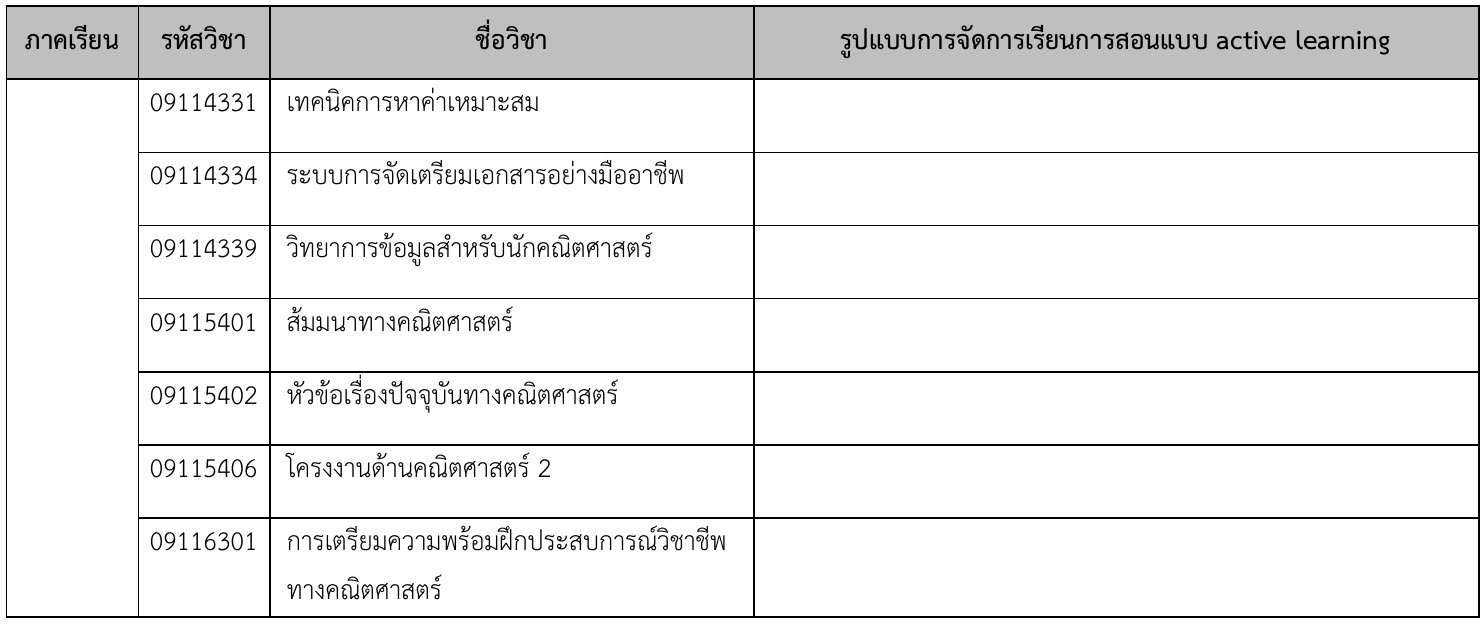
\includegraphics[width=1.05\textwidth]{Table3.3-2.jpg}
%\end{figure}
%\end{center}

\begin{doclist}
	\docitem{รายละเอียดของรายวิชา (มคอ. 3) }
	%\docitem{รูปแบบของการจัดการเรียนการสอนแบบ active learning ของแต่ละรายวิชาในหลักสูตร}
\end{doclist}


\subcriteria{The teaching and learning activities are shown to promote learning, learning how to learn, and instilling in students a commitment for life-long learning (e.g., commitment to critical inquiry, information-processing skills, and a willingness to experiment with new ideas and practices).}

หลักสูตรมีการกำหนด life-long learning ให้ครอบคลุมทักษะ 4 ด้าน คือ 
\begin{enumerate}
	\item การแก้ปัญหา
	\item การสื่อสาร
	\item การทำงานเป็นทีม
	\item การสืบค้น
\end{enumerate}
โดยมีตัวอย่างรายวิชาที่มีการจัดการเรียนการสอนเพื่อสนับสนุนส่งเสริมให้ผู้เรียนเกิดการเรียนรู้ตลอดชีวิต แสดงดังตาราง \ref{table:3.4-1}
{\small
	\begin{center}
		\begin{longtable}{|p{0.15\textwidth}|p{0.17\textwidth}|>{\raggedright}p{0.3\textwidth}|>{\raggedright\arraybackslash}>{}p{0.3\textwidth}|}
			\caption{การส่งเสริมและปลูกฝังการเรียนรู้ตอลดชีวิตของรายวิชาในหลักสูตร 2567}
			\label{table:3.4-1}\\
			\hline
			\multicolumn{1}{|c|}{\textbf{รายวิชา}} &
			\multicolumn{1}{c|}{\textbf{life-long learning}} &
			\multicolumn{1}{c|}{\textbf{วิธีการสอน}} &
			\multicolumn{1}{c|}{\textbf{วิธีการวัดประเมินผล}}\\
			\hline
			\endfirsthead	
			\caption {(ต่อ) การส่งเสริมและปลูกฝังการเรียนรู้ตอลดชีวิตของรายวิชาในหลักสูตร 2567}\\
			\hline
			\multicolumn{1}{|c|}{\textbf{รายวิชา}} &
			\multicolumn{1}{c|}{\textbf{life-long learning}} &
			\multicolumn{1}{c|}{\textbf{วิธีการสอน}} &
			\multicolumn{1}{c|}{\textbf{วิธีการวัดประเมินผล}}\\
			\hline
			\endhead	
			\hline\endfoot
			
			สัมมนาทางคณิตศาสตร์ประยุกต์&การแก้ปัญหา&
			จัดการเรียนการสอนโดยให้นักศึกษาต้องแก้ไขปัญหาเฉพาะหน้า เช่น การอธิบายแนวคิดที่ซับซ้อนให้ผู้อื่นเข้าใจได้ในเวลาจำกัด หรือการตอบคำถามที่ยังไม่มีคำตอบชัดเจน&ประเมินความสามารถในการอธิบาย หรือตอบคำถาม 	 
			\\ \cline{2-4}
			
			&การสื่อสาร &1. สอนการเขียนรายงานถอดบทเรียนของบทความวิจัยให้ถูกต้องตามหลักวิชาการ
			\newline 2. ให้นักศึกษานำเสนอถอดบทเรียนของบทความวิจัยต่อชั้นเรียน โดยเน้นความชัดเจน กระชับ และความ สามารถในการถ่ายทอดแนวคิดทางคณิตศาสตร์ที่ซับซ้อน
			&1. รายงานถอดบทเรียนของบทความวิจัย \newline 2. ประเมินความชัดเจนในการอธิบาย แนวคิดทางคณิตศาสตร์ ความสามารถในการใช้ภาษาที่เหมาะสม และการตอบคำถาม  \\ \cline{2-4}
			
			&การทำงานเป็นทีม &
			1. แบ่งกลุ่มนักศึกษาให้รับผิดชอบเตรียมความพร้อมของโสตทัศนูปกรณ์ และสถานที่ในการสัมมนาทุกสัปดาห์\newline 2. แบ่งกลุ่มนักศึกษาให้รับผิดชอบหน้าที่ต่างๆ ในการจัดทำรายงานฉบับสมบูรณ์ของถอดบทเรียนของบทความวิจัย & 1. ประเมินจากความสำเร็จของงานที่ได้รับมอบหมาย \newline 2. ประเมินจากรายงานการถอดบทเรียนของบทความวิจัยฉบับสมบูรณ์\\ \hline%\cline{2-4}
			
			& การสืบค้น
			& 1. สอนให้นักศึกษารู้จักแหล่งข้อมูลทางวิชาการที่น่าเชื่อถือ เช่น ฐานข้อมูลวารสารวิชาการ, Google Scholar\newline 2. สอนการใช้เครื่องมือ AI ในการสืบค้นข้อมูล   & ตรวจสอบความถูกต้อง ครบถ้วน และความน่าเชื่อถือของแหล่งข้อมูลที่นักศึกษานำมาใช้ในการนำเสนอ
			\\ \hline
			
			โครงงานด้านคณิตศาสตร์ประยุกต์& การแก้ปัญหา
			& ให้นักศึกษานำเสนอความก้าวหน้าของโครงงานต่ออาจารย์ที่ปรึกษาเป็นระยะ เพื่อระบุปัญหาและแนวทางในการแก้ปัญหา &ประเมินความสามารถในการระบุและวิเคราะห์ปัญหา การเลือกใช้วิธีการแก้ปัญหาที่เหมาะสม และความถูกต้องของผลลัพธ์ที่ได้
			
			\\ 	
			\cline{2-4}
			& การสื่อสาร
			& 1. สอนการเขียนรายงานทางวิชาการที่ถูกต้องตามหลักวิชาการ มีโครงสร้างชัดเจน และใช้ภาษาที่เข้าใจง่าย \newline 2. จัดกิจกรรมให้นักศึกษาฝึกนำเสนอโครงงานกับอาจารย์ที่ปรึกษาเพื่อเตรียมความพร้อมสำหรับการสอบโครงงาน โดยเน้นความชัดเจน การใช้สื่อ และความสามารถในการตอบคำถาม  & 1. รายงานโครงงานฉบับสมบูรณ์\newline 2. การสอบโครงงานทางคณิต ศาสตร์ประยุกต์
			\\ 	
			\cline{2-4}
			%\hline
			& การทำงานเป็นทีม	&1. กำหนดให้โครงงานเป็นลักษณะกลุ่ม โดยแต่ละกลุ่มจะต้องเลือกหัวข้อ วางแผน และดำเนินงานร่วมกัน\newline 2. จัดให้มีการติดตามความก้าวหน้าเป็นระยะ เพื่อติดตามความคืบหน้า ระบุปัญหา และช่วยในการแก้ไขกรณีเกิดความขัดแย้งหรือความไม่เข้าใจในทีม & 1. รายงานโครงงานฉบับสมบูรณ์ และการสอบโครงงานทางคณิตศาสตร์ประยุกต์\newline 2. ให้นักศึกษาแต่ละคนประเมินบทบาทของตนเองและเพื่อนร่วมทีมในด้านความรับผิดชอบ การมีส่วนร่วม และการสนับสนุนซึ่งกันและกัน 								
			%%%%%%%%%%%%
			%	\\ 
			%	\cline{2-4}
			\\ \hline
			& การสืบค้น	& ฝึกให้นักศึกษาใช้ AI เพื่อช่วยค้นหางานวิจัย งานที่เกี่ยวข้อง หรือวิธีการคำนวณในโครงงาน &  ตรวจสอบความถูกต้อง ครบถ้วน และความน่าเชื่อถือของแหล่งข้อมูลที่นักศึกษานำมาใช้ในการนำเสนอ						 \\
			\hline
			
		\end{longtable}
	\end{center}
	%%%%%%%%%%%%%%
	
	
	
	
	
	
	\begin{doclist}
		\docitem{รายละเอียดของรายวิชา (มคอ.3) รายวิชาสัมมนาทางคณิตศาสตร์ประยุกต์}
		\docitem{รายละเอียดของรายวิชา (มคอ.3) รายวิชาโครงงานด้านคณิตศาสตร์ประยุกต์}
		\docitem{รายงานการประชุมอาจารย์ผู้รับผิดชอบหลักสูตร/อาจารย์ประจำสาขาวิชาเกี่ยวกับการจัดการเรียนการสอน Life-Long Learning ของหลักสูตร}
	\end{doclist}


%%%%%%%%%%%%%%%%3.5 %%%%%%%%%%%%%%%%%%%%%%%%%%%%%%
\subcriteria{The teaching and learning activities are shown to inculcate in students, new ideas, creative thought, innovation, and an entrepreneurial mindset.}
หลักสูตรมุ่งเน้นการพัฒนานักศึกษาให้มีความคิดสร้างสรรค์และมีแนวคิดเชิงนวัตกรรม ผ่านกิจกรรมการเรียนการสอนที่เน้นการลงมือปฏิบัติจริง 
เพื่อปลูกฝังกรอบความคิด (Mindset) 4 ด้านที่สำคัญให้แก่นักศึกษา ดังนี้
\begin{enumerate}
	\item ความคิดใหม่ ๆ (New Ideas) ส่งเสริมการคิดค้นแนวคิดที่แตกต่างและไม่ลอกเลียนแบบ
	\item ความคิดสร้างสรรค์ (Creative Thought) กระตุ้นการคิดนอกกรอบและแก้ไขปัญหาด้วยวิธีการใหม่ ๆ
	\item นวัตกรรม (Innovation) พัฒนาผลงานหรือกระบวนการที่สามารถนำไปใช้แก้ปัญหาและสร้างมูลค่าเพิ่มได้จริง
	\item แนวคิดแบบผู้ประกอบการ (Entrepreneurial Mindset) สร้างทักษะการวางแผนธุรกิจ การจัดการความเสี่ยง และการมองหาโอกาสทางธุรกิจ
\end{enumerate}
หลักสูตรใช้ 4 รายวิชาหลักเป็นกลไกในการขับเคลื่อนการพัฒนาทักษะดังกล่าว โดยมีรายละเอียดดังนี้
\begin{enumerate}
	\item รายวิชา 00-100-301 ความเป็นผู้ประกอบการ
	\begin{itemize}
		\item เนื้อหา \\สอนหลักการเป็นผู้ประกอบการ การวิเคราะห์แนวโน้มธุรกิจ และการสร้างแบบจำลองธุรกิจ (Business Model Canvas)
		\item กิจกรรมการเรียนการสอน \\ใช้กระบวนการ Active Learning และ Design Thinking ให้นักศึกษาได้ฝึกวิเคราะห์ สร้างไอเดียธุรกิจใหม่ พัฒนาต้นแบบผลิตภัณฑ์ และฝึกนำเสนอแผนธุรกิจ (Pitching)
	\end{itemize}
		\item รายวิชา 09-116-301 การเตรียมความพร้อมฝึกประสบการณ์วิชาชีพทางคณิตศาสตร์ประยุกต์ และรายวิชา 09-116-402 สหกิจศึกษาทางคณิตศาสตร์ประยุกต์
	\begin{itemize}
		\item เนื้อหา \\เน้นการฝึกประสบการณ์วิชาชีพในสถานประกอบการจริง
		\item ให้นักศึกษาได้เรียนรู้จากการทำงานจริง และได้รับแรงบันดาลใจจากผู้ประกอบการและศิษย์เก่าที่ประสบความสำเร็จ เพื่อนำประสบการณ์มาประยุกต์ใช้ในการสร้างสรรค์นวัตกรรมในบริบททางธุรกิจ
	\end{itemize}
		\item รายวิชา 09-115-404 รายวิชาโครงงานด้านคณิตศาสตร์ประยุกต์
	\begin{itemize}
		\item เนื้อหา \\ให้นักศึกษาบูรณาการความรู้ทางคณิตศาสตร์เพื่อสร้างโครงงานที่แก้ไขปัญหาในชีวิตจริงหรือภาคธุรกิจ
		\item กิจกรรมการเรียนการสอน \\นักศึกษาทำงานเป็นกลุ่มเพื่อพัฒนาโครงงาน ตั้งแต่การเสนอหัวข้อ ออกแบบ พัฒนา และนำเสนอผลงาน
		\item ตัวอย่างโครงงานที่โดดเด่น
		\begin{itemize}
			\item นวัตกรรมด้านการเงิน \\ ``การลงทุนในหุ้นร่วมกับออปชั่น" เพื่อลดความเสี่ยงในการลงทุน
			\item นวัตกรรมเชิงสร้างสรรค์ \\``การสร้างรูปแบบดนตรีผ่านระบบพลวัตแบบโกลาหล (Chaotic System)" ซึ่งได้ต่อ ยอดไปสู่การนำเสนอในเวทีประชุมวิชาการทางคณิตศาสตร์ ครั้งที่ 29 ประจำปี 2568 (AMM2025) ภายใต้หัวข้อ  “Lead a better future with Mathematics” ระหว่างวันที่ 21-23 พฤษภาคม 2568 ณ โรงแรม ดิ เอมเมอรัลด์ - กรุงเทพฯ
			\item นวัตกรรมเพื่อสังคม\\``การพัฒนาเว็บไซต์ต้นแบบสำหรับคัดกรองโรคอัลไซเมอร์" โดยใช้การถดถอยโลจิสติก
			\item นวัตกรรมด้านธุรกิจ\\``การวางแผนจัดส่งสินค้าหลายวันจากหลายคลัง" เพื่อเพิ่มประสิทธิภาพด้านโลจิสติกส์ ซึ่งได้รับรางวัลเหรียญทองแดงจากการประชุมวิชาการระดับปริญญาตรีด้านคณิตศาสตร์ประยุกต์ ครั้งที่ 13 (UAMC2025) วันอาทิตย์ที่ 30 มีนาคม 2568 สถาบันเทคโนโลยีพระจอมเกล้าเจ้าคุณทหารลาดกระบัง 
			\end{itemize}
		\end{itemize}
\end{enumerate}



 
\begin{doclist}
	\docitem{รายละเอียดของรายวิชา (มคอ.3) รายวิชาที่ส่งเสริมแนวคิดการสร้างนวัตกรรมและแนวคิดความเป็นผู้ประกอบการ}
	\docitem{หลักฐานการเข้าร่วมงานประชุมวิชาการของนักศึกษา}
\end{doclist}

\subcriteria{The teaching and learning processes are shown to be continuously improved to ensure their relevance to the needs of industry and are aligned to the expected learning outcomes.}
หลักสูตรได้ดำเนินการปรับปรุงกระบวนการและกลยุทธ์การจัดการเรียนการสอนอย่างต่อเนื่อง เพื่อตอบสนองต่อความต้องการของตลาดแรงงานและภาคอุตสาหกรรม รวมถึงเพื่อส่งเสริมให้นักศึกษาเกิดการเรียนรู้ที่สอดคล้องกับ ผลลัพธ์การเรียนรู้ของหลักสูตร (PLOs) 

ในภาคเรียนที่ 1 ปีการศึกษา 2567 จากการออกนิเทศนักศึกษาฝึกสหกิจที่บริษัท บริษัท Western Digital Storage Technologies (Thailand) ทางบริษัทมีข้อเสนอแนะว่า ในรายวิชาทางด้านประยุกต์ของหลักสูตร เช่น การสร้างแบบจำลองทางคณิตศาสตร์เบื้องต้น การเขียนโปรแกรมคอมพิวเตอร์ทางคณิตศาสตร์ เทคนิคการหาค่าเหมาะสม และวิทยาการข้อมูลสำหรับนักคณิตศาสตร์  หลักสูตรควรนำนักศึกษาไปศึกษาดูงานในสถานประกอบการ เพื่อเข้าใจบริบทการทำงาน และเห็นการประยุกต์ใช้คณิตศาสตร์ในโลกอุตสาหกรรม และอาจารย์ผู้สอนควรสนับสนุนให้นักศึกษาสอบวัดระดับความ
สามารถด้านการเรียนรู้เชิงลึกจากองค์กรหรือหน่วยงานที่ได้รับการยอมรับในระดับสากล (Certificate)

อาจารย์ผู้สอนในรายวิชา ได้นำข้อเสนอแนะมาปรับปรุงกระบวนการจัดการเรียนการสอนซึ่งระบุไว้ใน มคอ.3 ของรายวิชาในภาคเรียนที่ 2 ปีการศึกษา 2567 ซึ่งมีรายละเอียดดังนี้
\begin{enumerate}
	\item ในรายวิชาการสร้างแบบจำลองทางคณิตศาสตร์เบื้องต้น รายวิชาการเขียนโปรแกรมคอมพิวเตอร์ทางคณิตศาสตร์ และรายวิชาเทคนิคการหาค่าเหมาะสม กำหนดจัดกิจกรรมศึกษาดูงานร่วมกัน
	\item ในรายวิชาวิทยาการข้อมูลสำหรับนักคณิตศาสตร์ ปรับปรุงกิจกรรมการเรียนการสอนโดยส่งเสริมให้นักศึกษาสอบวัดระดับความสามารถด้านการเรียนรู้เชิงลึกจากองค์กรหรือหน่วยงานที่ได้รับการยอมรับในระดับสากล (Certificate)
\end{enumerate}
ซึ่งมีผลการดำเนินงานดังนี้
\begin{enumerate}
	\item มีการนำนักศึกษาไปศึกษาดูงาน ณ บริษัท บ้านปู จำกัด (มหาชน) เมื่อวันที่ 11 กุมภาพันธ์ 2568 ซึ่งนักศึกษาได้เรียนรู้เกี่ยวกับการประยุกต์ใช้คณิตศาสตร์ในธุรกิจและอุตสาหกรรม
	\item นักศึกษาทุกคนที่ลงทะเบียนเรียนรายวิชาวิทยาการข้อมูลสำหรับนักคณิตศาสตร์ จำนวน 16 คน ได้รับใบประกาศนียบัตรอย่างน้อยหนึ่งใบ
	จาก IBM คิดเป็นร้อยละ 100
\end{enumerate}

\begin{doclist}
	\docitem{ภาพกิจกรรมโครงการศึกษาดูงาน}
	\docitem{รายละเอียดของรายวิชา (มคอ.3) รายวิชาการสร้างแบบจำลองทางคณิตศาสตร์เบื้องต้น}
	\docitem{รายละเอียดของรายวิชา (มคอ.3) การเขียนโปรแกรมคอมพิวเตอร์ทางคณิตศาสตร์ }
	\docitem{รายละเอียดของรายวิชา (มคอ.3) เทคนิคการหาค่าเหมาะสม}
	\docitem{รายละเอียดของรายวิชา (มคอ.3) วิทยาการข้อมูลสำหรับนักคณิตศาสตร์}
	\docitem{ใบ Certificate ของนักศึกษา}
\end{doclist}

